\documentclass[12pt,a4paper]{article}

% --- Packages ---
\usepackage{geometry}
\geometry{margin=1in}
\usepackage{setspace}
\setstretch{1.3}
\usepackage{fancyhdr}
\usepackage{graphicx}
\usepackage{listings}
\usepackage{xcolor}
\usepackage{caption}
\usepackage{pgfplots}
\pgfplotsset{compat=1.17}
\usepackage{pgf-pie}
\usepackage{longtable}
\usepackage{hyperref}

% --- Header / Footer ---
\pagestyle{fancy}
\fancyhead[L]{Library Management System}
\fancyhead[R]{Page \thepage}
\fancyfoot{}

% --- Code listing style ---
\definecolor{backcolour}{rgb}{0.95,0.95,0.92}
\definecolor{keywordcolour}{rgb}{0.0,0.0,0.6}
\definecolor{stringcolour}{rgb}{0.58,0.0,0.82}
\definecolor{commentcolour}{rgb}{0.0,0.5,0.0}
\lstdefinestyle{pyStyle}{
    backgroundcolor=\color{backcolour},
    commentstyle=\color{commentcolour},
    keywordstyle=\color{keywordcolour}\bfseries,
    stringstyle=\color{stringcolour},
    basicstyle=\ttfamily\small,
    breaklines=true,
    numbers=left,
    numberstyle=\tiny,
    captionpos=b,
    frame=single,
    showstringspaces=false
}
\lstset{style=pyStyle, language=Python}

% --- Title ---
\title{\textbf{Library Management System}\\[5pt]\large Python Console Application}
\author{Manas (main.py, utils.py) \\ Piyush (book\_operations.py, manage\_books.py) \\ Smit (helpers.py, storage.py)}
\date{\today}

\begin{document}

\maketitle
\thispagestyle{empty}

\begin{abstract}
This document describes a simple Library Management System implemented in Python. The program is modularized across six files so that three team members can work in parallel. It supports adding, viewing, searching, deleting, and persisting book records (JSON). Example charts illustrate simple dataset summaries.
\end{abstract}

\newpage
\tableofcontents
\newpage

\section{Introduction}
The Library Management System is a lightweight console application that enables basic CRUD operations (Create, Read, Update, Delete) for book records, and persists data into a JSON file. The project demonstrates modular programming, file I/O, unique ID generation, and simple team collaboration via Git.

\section{Project Structure}
\begin{longtable}{|p{4cm}|p{9cm}|}
\hline
\textbf{File} & \textbf{Purpose} \\ \hline
\texttt{main.py} & Program entry point; menu and control flow. \\ \hline
\texttt{book\_operations.py} & Add and view books. \\ \hline
\texttt{manage\_books.py} & Search and delete books. \\ \hline
\texttt{helpers.py} & Small helper functions (confirmation, display). \\ \hline
\texttt{storage.py} & Load and save JSON data. \\ \hline
\texttt{utils.py} & Utility functions (ID generator). \\ \hline
\end{longtable}

\section{How to Run}
\begin{enumerate}
    \item Upload all Python files into one folder (local or repository).
    \item Ensure Python 3 is installed.
    \item Run from terminal:
    \begin{verbatim}
    python main.py
    \end{verbatim}
    \item Follow the on-screen menu.
\end{enumerate}

\section{Code Listings}
Below are the source files. (You can copy these into `.py` files.)

\subsection{main.py}
\begin{lstlisting}[caption=main.py]
from book_operations import add_book, view_books
from manage_books import search_book, delete_book
from storage import save_data, load_data

def main():
    books = load_data()

    while True:
        print("\n=== Library Management System ===")
        print("1. Add Book")
        print("2. View Books")
        print("3. Search Book")
        print("4. Delete Book")
        print("5. Save & Exit")

        choice = input("Enter your choice: ")

        if choice == '1':
            add_book(books)
        elif choice == '2':
            view_books(books)
        elif choice == '3':
            search_book(books)
        elif choice == '4':
            delete_book(books)
        elif choice == '5':
            save_data(books)
            print("✅ Data saved! Exiting...")
            break
        else:
            print("❌ Invalid choice, try again!")

if __name__ == "__main__":
    main()
\end{lstlisting}

\subsection{book\_operations.py}
\begin{lstlisting}[caption=book_operations.py]
from utils import generate_id

def add_book(books):
    title = input("Enter book title: ")
    author = input("Enter author name: ")
    year = input("Enter publication year: ")
    book_id = generate_id()

    book = {"id": book_id, "title": title, "author": author, "year": year}
    books.append(book)
    print("�� Book added successfully!")

def view_books(books):
    if not books:
        print("No books found in the library.")
        return
    print("\n--- Library Books ---")
    for b in books:
        print(f"ID: {b['id']} | {b['title']} by {b['author']} ({b['year']})")
\end{lstlisting}

\subsection{manage\_books.py}
\begin{lstlisting}[caption=manage_books.py]
def search_book(books):
    keyword = input("Enter title or author to search: ").lower()
    results = [b for b in books if keyword in b["title"].lower() or keyword in b["author"].lower()]
    if results:
        print("\n--- Search Results ---")
        for b in results:
            print(f"{b['id']} - {b['title']} by {b['author']} ({b['year']})")
    else:
        print("❌ No books found matching your search.")

def delete_book(books):
    book_id = input("Enter book ID to delete: ")
    for b in books:
        if b["id"] == book_id:
            books.remove(b)
            print("��️ Book deleted successfully!")
            return
    print("❌ No book found with that ID.")
\end{lstlisting}

\subsection{helpers.py}
\begin{lstlisting}[caption=helpers.py]
def confirm_action(message):
    choice = input(f"{message} (y/n): ").lower()
    return choice == 'y'

def display_line():
    print("=" * 40)
\end{lstlisting}

\subsection{storage.py}
\begin{lstlisting}[caption=storage.py]
import json
import os

FILE_NAME = "books.json"

def load_data():
    if not os.path.exists(FILE_NAME):
        return []
    with open(FILE_NAME, "r") as f:
        return json.load(f)

def save_data(books):
    with open(FILE_NAME, "w") as f:
        json.dump(books, f, indent=4)
\end{lstlisting}

\subsection{utils.py}
\begin{lstlisting}[caption=utils.py]
import uuid

def generate_id():
    return str(uuid.uuid4())[:8]
\end{lstlisting}

\section{Sample Dataset (Example)}
Below is an example dataset (this is what might appear in \texttt{books.json}):

\begin{verbatim}
[
  {"id": "a1b2c3d4", "title": "Python Basics", "author": "John Doe", "year": "2023"},
  {"id": "e5f6g7h8", "title": "Data Science 101", "author": "Alice Smith", "year": "2023"},
  {"id": "i9j0k1l2", "title": "Intro to ML", "author": "Robert Lee", "year": "2022"}
]
\end{verbatim}

\section{Data Visualization (Example Figures)}
These charts use the example dataset above and are included for report visuals.

\subsection{Bar Chart: Books by Year}
\begin{center}
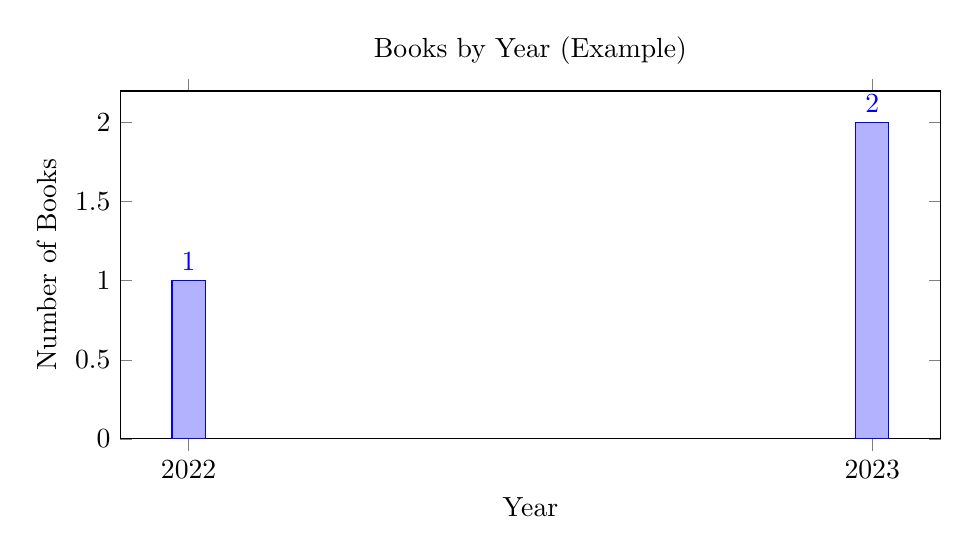
\begin{tikzpicture}
\begin{axis}[
    ybar,
    xlabel={Year},
    ylabel={Number of Books},
    ymin=0,
    symbolic x coords={2022,2023},
    xtick=data,
    nodes near coords,
    width=12cm,
    height=6cm,
    bar width=12pt,
    title={Books by Year (Example)}
]
\addplot coordinates {(2022,1) (2023,2)};
\end{axis}
\end{tikzpicture}
\captionof{figure}{Example bar chart showing number of books by year.}
\end{center}

\subsection{Pie Chart: Distribution by Author}
\begin{center}
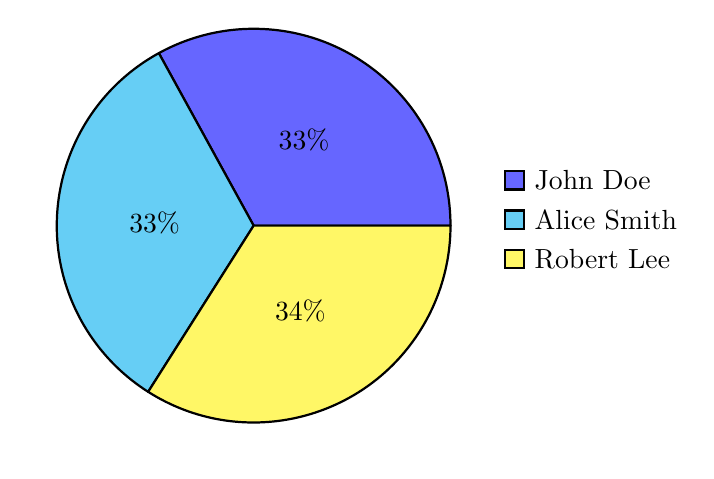
\begin{tikzpicture}
\pie[text=legend, radius=2.5]{
33/John Doe,
33/Alice Smith,
34/Robert Lee
}
\end{tikzpicture}
\captionof{figure}{Example pie chart showing distribution of books by author.}
\end{center}

\section{Sample Console Output}
\begin{verbatim}
=== Library Management System ===
1. Add Book
2. View Books
3. Search Book
4. Delete Book
5. Save & Exit
Enter your choice: 1
Enter book title: Python Basics
Enter author name: John Doe
Enter publication year: 2023
�� Book added successfully!
\end{verbatim}

\section{Future Enhancements}
\begin{itemize}
    \item Add GUI using Tkinter or PyQt.
    \item Implement user roles (admin, student).
    \item Add loan/return tracking and due dates.
    \item Add CSV/Excel import-export.
\end{itemize}

\section{Acknowledgements}
Thanks to Manas, Piyush, and Smit for collaborating on code and documentation.

\bigskip
\noindent\textbf{Notes for Overleaf:}
\begin{itemize}
    \item This file uses \texttt{pgfplots} and \texttt{pgf-pie}. Overleaf includes these packages by default.
    \item If charts do not render, ensure the project compiles with PDFLaTeX and check package availability.
\end{itemize}

\end{document}
